\chapter{Umsetzung}
\label{chap:implementierung}
Auf Basis welcher Methodiken und Ansätze die relevanten Informationen extrahiert werden können, wurde in Kapitel \ref{sec:literaturueberblick} dargestellt. Nun gilt es diese Ansätze in einem System zu implementiert. In diesem Kapitel werden die Funktionalitäten der Pipeline zusammengetragen. Dabei werden verwendete Technologien und Implementationsaspekte genauer beschrieben.
\section{Beschreibung}
Damit alle Ansätze und Methoden zur Extraktion von Informationen gut funktionieren und vergleichbar bleiben, wird eine Übersetzungsfunktion der \emph{Bedarfsmeldungen} hinzugefügt. Auch wenn die \emph{Bedarfsmeldungen} in den meisten Fällen auf Deutsch sind, hilf es diese zu übersetzen, damit keine Unterschiede in der Ergebnisqualität resultiert, da einige Methoden und Ansätze auf Basis von Englischen Trainingssätzen trainiert wurden. Schließlich müssen alle aus Kapitel \ref{sec:literaturueberblick} untersuchten Ansätze implementiert und nutzbar sein. Sie sollen die Möglichkeit haben \emph{Bedarfsmeldungen} als Input zu erhalten und eine strukturierte \emph{Bedarfsmeldung} als Ausgabe zurückzugeben. Zur vereinfachten Entwicklung soll das System modular sein, damit Methoden und Ansätze nach belieben durchgetauscht und verwendet werden können.\\
\section{Konkreter Ablauf der Pipeline}
Dieses Kapitel beschreibt den Ablauf der Pipeline. Dazu wird das Aktivitätsdiagramm aus der Abbildung \ref{fig:ablaufsystemabstrakt} verfeinert und mit allen analysierten Komponenten aus Kapitel \ref{sec:literaturueberblick} genauer beschrieben.
\begin{figure}[H]
	\centering  
	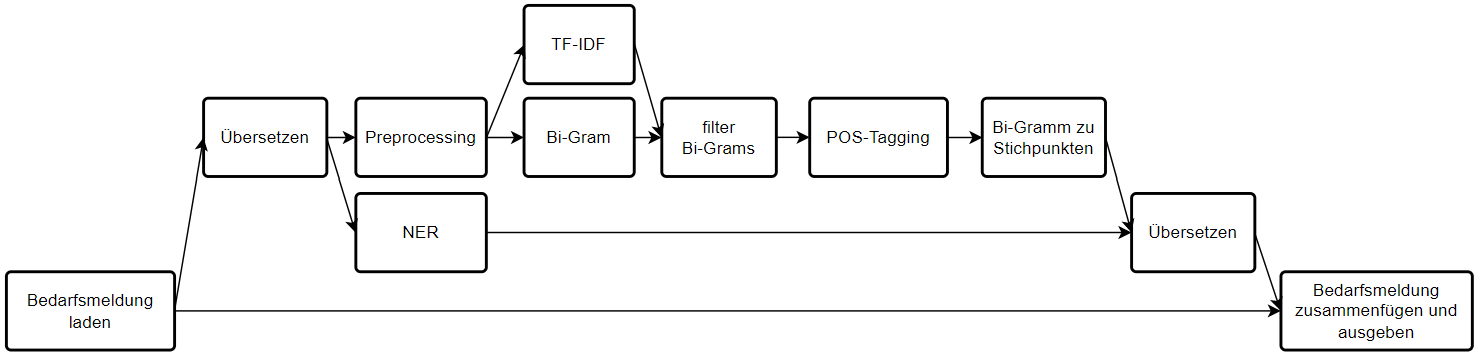
\includegraphics[width=\linewidth]{Abbildungen/flowchart.png}
	\caption{Flussdiagramm der Pipeline.}
	\label{fig:flowchart}
\end{figure}\mbox{} \\
Die Abbildung \ref{fig:flowchart} zeigt das UML-Aktivitätsdiagramm der Python Pipeline zur Strukturierung von \emph{Bedarfsmeldungen}. Im ersten Schritt \emph{unstrukturierte Bedarfsmeldung strukturieren} im Ablauf der Pipeline wird eine \emph{Bedarfsmeldung} ausgewählt und in die festgelegte \emph{Bedarfsmeldungsstruktur} aus Kapitel \ref{sec:strukturierungbedarfsmeldung} umgebaut. Die Felder \emph{Einsatzbeginn} und \emph{Einsatzende} werden zu einem Feld \emph{Einsatz} zusammengefügt. Neben den Feldern \emph{Aufgaben} und \emph{Skills} bleiben alle weiteren Felder bis zum letzten Punkt Ausgabe unverändert. Die Felder \emph{Aufgaben} und \emph{Skills} werden jeweils in die Schleife weitergeleitet, wo sie auf Stichpunkte reduziert werden. Der Prozess zur Reduktion durchläuft mehrere Schritte. Zu Beginn werden die Volltexte aus den Feldern im Punkt \emph{ins Englische übersetzen} übersetzt. Anschließend erfolgt im Schritt \emph{Datums-Daten und Zeiten mit NER extrahieren} zum einen die Extrahierung der zeitbezogenen Daten. Darauffolgend wird der Volltext im Punkt \emph{Preprocessing} für die weitere Nutzung vorverarbeitet. Der Grund warum die Extraktion mit \emph{NER} nicht nach der Vorverarbeitung durchgeführt werden kann ist, da im Vorverarbeitungsschritt alle Nummern und somit auch alle zeitbezogenen Daten entfernt werden. Die Resultate des \emph{NER} werden zum Ende hin zurück ins deutsche übersetzt und der fertigen Stichpunktliste beigefügt. Zur Erstellung der Stichpunktliste werden relevante Schlüsselwörter durch die \emph{TF-IDF}-Methode ermittelt. Anschließend wird der vorverarbeitete Text zu \emph{Bi-Grammen} umgeformt. Beim Punkt \emph{Bi-Gramme auf Schlüsselwörter filtern} werden alle \emph{Bi-Gramme} entfernt, die kein Schlüsselwort aus der \emph{TF-IDF}-Methode enthalten. Somit erhält der Schritt \emph{untypische Wortartenkombinationen mit POS-Tagging entfernen} eine reduzierte Liste mit \emph{Bi-Grammen}, bei dem mindestens eines der beiden \emph{Bi-Gramm}-Wörter ein Schlüsselwort Wort darstellt. Jedes Wort der \emph{Bi-Gramm}-Liste durchläuft eine weitere Filterung. Im Englischen existieren Wortarten, die typischerweise nicht nebeneinander stehen. Durch Entfernung dieser \emph{Bi-Gramme} durch POS-Tagging-Kombinationen erfolgt eine weitere Trennung der Wortketten in der \emph{Bi-Gramm}-Liste. Wörter die nicht zusammengehören, verlieren dadurch die Verbindung zueinander. Im darauf folgenden Schritt \emph{Bi-Gramm zu Stichpunkten überführen} werden die \emph{Bi-Gramme} jeweils zu einem String zusammengefügt, bei dem im darauf Folgendem \emph{Bi-Gramm} ebenfalls ein relevantes Wort enthalten sind. Dadurch formt sich eine Liste mit Stichpunkten bestehend aus eins bis x vielen Wörtern, die Bezug zueinander haben. Im Schritt \emph{ins Deutsche übersetzen} wird die Liste mit Stichpunkten zurück ins übersetzt. Dieser Ablauf wird für die beiden Felder \emph{Aufgaben} und \emph{Skills} durchlaufen, da diese Volltextfelder darstellen.
\section{Implementationsdetails}
Dieses Kapitel beschreibt den technischen Entwicklungsprozess zur Umsetzung der Anforderungen des Systems. Die Implementierung fokussiert sich auf die Umsetzungen von Technologien und Funktionsweisen verschiedener Anforderungen. Zudem wird die Struktur des Projektes aufgezeigt.
\subsection{Pipeline}
Die Pipeline wurde in der Programmiersprache Python umgesetzt. Python hat sich zu einer der populärsten interpretierten Programmiersprachen entwickelt \cite{mckinney2012python}. Die Programmiersprache eignet sich insbesondere für die Erstellung kleiner Programme und Skripte, die zur Automatisierung von Aufgaben eingesetzt werden können \cite{mckinney2012python}. Python hat eine große und aktive Community für wissenschaftliche Berechnungen und Datenanalysen hervorgebracht und hat sich in den letzten Jahren zu einer der wichtigsten Sprachen für Data Science, maschinelles Lernen und allgemeine Softwareentwicklung in Wissenschaft und Industrie entwickelt \cite{mckinney2012python}. Python unterstützt Modularität, wodurch ein Teil der Anforderungen somit abgedeckt werden kann. Die Implementierungen der einzelnen Verfahren aus den Anforderungen werden nicht manuell, sondern auf Basis von bereits existierende Bibliotheken umgesetzt.
\subsection{Projektstruktur}
\label{sec:projektstruktur}
Das Projekt wird in einem git Repository gespeichert und versioniert. Die Projektstruktur ist ohne zusätzliche Konfigurationsdateien wie folgt aufgebaut:
\dirtree{%
	.1 .git/.
	.2 modules/.
	.3 ner.py.
	.3 nGram.py.
	.3 posTagging.py.
	.3 preprocessing.py.
	.3 readRequirements.py.
	.3 textRankingAlgorithm.py.
	.3 tfIdf.py.
	.3 transformRequirements.py.
	.3 translate.py.
	.2 requirements/.
	.3 jiraTickets.json.
	.3 preprocessedRequirements.json.
	.3 ....
	.2 app.py.
	.2 ....
}
Die einzelnen Module aus dem Flussdiagramm in Kapitel \ref{fig:flowchart} sind im Verzeichnis \url{modules/} in separaten \url{.py} Dateien gelagert. Die \emph{Bedarfsmeldungen} werden im \url{requirements/}-Verzeichnis gespeichert. Alle relevanten \emph{Bedarfsmeldungen} sind in der \url{jiraTickets.json}-Datei in einer Liste gespeichert. Die Datei \url{app.py} ist der Kern der Pipeline. Diese importiert alle Module und implementiert die Struktur der Pipeline. Das Projekt kann über den Befehl \lstinline{> py app.py} ausgeführt werden.
\subsection{Modulimplementationen}
Nachfolgend werden Implementationsdetails zu den einzelnen Modulen gegeben. Dabei werden verwendete Bibliotheken und Code-Details näher erläutert.
\paragraph{Strukturierung von Bedarfsmeldungen}\mbox{}\\
Die \emph{Bedarfsmeldungen} wurden über die Jira-Schnittstelle extrahiert und im Verzeichnis \url{requirements/jiraTickets.json} gespeichert. Zur Eingrenzung der Datenmenge wurde ein Filter angewendet, der nur die \emph{offenen} und \emph{eskalierten} \emph{Bedarfsmeldungen} zurückgibt. Diese sind die relevanten und noch aktuellen \emph{Bedarfsmeldungen}. Zudem wurden alle unrelevanten Felder mit einem weiteren Filter herausgenommen. Die Daten aus der Jira-API bestehen namentlich aus \emph{customfields} mit einer angehangenden ID. Der Softwareprototyp lädt in dem Modul \emph{readRequirements.py} die unstrukturierten Fields und formt diese in dem Modul \emph{transformRequirements.py} in \emph{Bedarfsmeldungs}-Objekte um.
\begin{center}
	\begin{tabularx}{1\textwidth} { 
			| >{\raggedright\arraybackslash}X 
			| >{\raggedright\arraybackslash}X
			| >{\raggedright\arraybackslash}X | }
		\hline
		Display-Felder & Jira-API-Felder & Objekt-Felder \\
		\hline
		\hline
		Überschrift & summary & header\\
		\hline
		Rolle & customfield\_15321 & role\\
		\hline
		Aufgaben & customfield\_10288 & tasks\\
		\hline
		Skills & customfield\_10296 & skills\\
		\hline
		Skill-Level & customfield\_15322 & skillLevel\\
		\hline
		Kunde & customfield\_10279 & customer\\
		\hline
		Einsatzort & customfield\_10297 & location\\
		\hline
		Beginn & customfield\_10293 & timePeriod\\
		\hline
		Ende & customfield\_10294 & timePeriod\\
		\hline
		Tagessatz & customfield\_10298 & dailyRate\\
		\hline
	\end{tabularx}\\
	\captionof{table}{Übersicht der Datenfelder}
	\label{tab:jiradaten}
\end{center}
In der Tabelle \ref{tab:jiradaten} ist in der ersten Spalte eine Übersicht der Datenfelder, wie diese in der Abbildung \ref{fig:jiraafter} mit dem Mockup einer standardisierten \emph{Bedarfsmeldung} auftauchen. In der zweiten Spalte sind die dazugehörigen Feldernamen, die in der \url{jiraTickets.json} enthalten sind. Die dritte Spalte spiegelt die jeweiligen Namen innherhalb des  \emph{Bedarfsmeldungs}-Objekts im Prototypen wieder. Das  \emph{Bedarfsmeldungs}-Objekt dient der strukturierten Handhabung der \emph{Bedarfsmeldungs}-Daten innerhalb des Systems.

%Um einen Freitext aus einer einzelnen \emph{Bedarfsmeldung} für die Pipeline zu laden werden Daten mit der Endung \url{.txt} verwendet.
%\begin{lstlisting}[caption={Implementation der Methode read() des Moduls \emph{readRequirements.py}}, label=lst:read]
%	def read(filename):
%		path = os.path.join(PATH, filename)
%		file = open(path, "r", encoding="utf-8")
%		content = file.read()
%		file.close()
%		return content
%\end{lstlisting}
%Im Listing \ref{lst:read} ist die Implementierung der Methode zum laden eines Freitextes dargestellt. Durch ein mitgelieferten Parameter \emph{filename} wird der Name der Datei in Zeile 2 an den Pfad angehängt. Mit der Methode \lstinline{open()}
%aus Zeile 3 kann die Datei geladen werden. Die Methode erhält die Parameter Pfad, \emph{'r'} (read) und das encoding \emph{'utf-8'}. Das encoding ist dabei Entscheidend, damit die unstrukturierten \emph{Bedarfsmeldungen} laden können. Bei der Pflege in Jira wird wenig Wert auf eine einheitliche Struktur. Somit können Zeichen enthalten sein, die beim öffnen nicht erkannt werden und eine Fehlermeldung wird zurückgegeben. Zur Vermeidung dieses Fehlers wird das encoding festgelegt. Nach dem laden durch die Methode \lstinline{read()} wird der Inhalt der \url{.txt} Datei in der Variable \emph{content} gespeichert und zurückgegeben.
\paragraph{Übersetzung}\mbox{}\\
Das Modul \emph{translate.py} ist dazu da, um die \emph{Bedarfsmeldungen} zu übersetzen. Für die Übersetzung wurde die Python Bibliothek \emph{deep-translator} verwendet. Diese bietet Implementationen unterschiedlicher Übersetzungs-APIs von diversen Anbietern. Der Vorteil ist dabei die vereinfachte Möglichkeit Anbieter bei Bedarf zu wechseln.
%\begin{lstlisting}[caption={Implementation des Moduls \emph{translate.py}}, label=lst:translate]
%	from deep_translator import GoogleTranslator
%	
%	def translate(text):
%		translated = GoogleTranslator(source='auto', target='en').translate(text)
%		return translated
%\end{lstlisting}
%Das Listing \ref{lst:translate} zeigt die Implementation des Moduls. 
Es wurde sich für den Google Translator entschieden, da hierfür kein API-Key benötigt wird. Die Methode erhält einen Text als Parameter. Der Google Translator erhält die Parameter \emph{source} und \emph{target}, beidem \emph{source} angibt in welcher Sprache der Eingabetext ist. Durch Angabe von \emph{'auto'} wird die Sprache ermittelt. Der Grund dafür ist, dass grundsätzlich anderssprachige \emph{Bedarfsmeldung} enthalten sein können. Der Parameter \emph{target} ist die Zielsprache in welche der Input übersetzt werden soll. Die Zielsprache ist hier Englisch (\emph{'en'}).
\paragraph{NER}\mbox{}\\
Um die Methode \emph{NER} zu Implementieren wurde die Bibliothek \emph{spaCy} und das Modell \emph{en\_core\_web\_sm} verwendet. 
%\begin{lstlisting}[caption={Implementation des Moduls \emph{ner.py}}, label=lst:ner]
%	import spacy
%	nlp = spacy.load("en_core_web_sm")
%	ner_categories = ["ORG","FAC","GPE","PRODUCT", "EVENT", "LANGUAGE", "DATE", "QUANTITY"]
%	def useNER(requirement):
%		tokenized = nlp(requirement)
%		entities = []
%		for ent in tokenized.ents:
%			if ent.label_ in ner_categories:
%				entities.append((ent.text, ent.label_))
%	return entities
%\end{lstlisting}
Die zu extrahierende Kategorie ist Datum (DATE). Innerhalb der Methode \lstinline{useNER()} wird der Volltext als Parameter übergeben und zu Tokens umgeformt. Anschließend werden alle Tokens durchlaufen und nach ihren Kategorien überprüft. Ist ein Token die definierte Kategorie, wird der Token in eine separate Liste gespeichert und zurückgegeben. Die extrahierten Tokens werden aus dem Volltext entfernt, um am ende keine doppelten Stichpunkte zu erhalten.
\paragraph{Preprocessing}\mbox{}\\
Vor der weiteren Nutzung der Daten innerhalb einer \emph{Bedarfsmeldung}, ist es erforderlich diese von irrelevanten Wörtern, Zeichen und Formatierungen zu befreien.% Zur Entfernung von Satzzeichen wurde die Bibliothek \emph{string} verwendet.
%\begin{lstlisting}[caption={Implementation der Methode removePunctuation() des Moduls \emph{preprocessing.py}}, label=lst:punctuation]
%	import string
%	def removePunctuation(text):
%		content=""
%		for i in text: 
%			if i not in string.punctuation:
%				content+=i    
%		return content
%\end{lstlisting}
%Im Listing \ref{lst:punctuation} ist die Implementierung dargestellt. Die \emph{Bedarfsmeldung} wird in Zeile 2 als Parameter übergeben. In Zeile 4 erfolgt ein Durchlauf jedes Zeichens innerhalb der \emph{Bedarfsmeldung}. Falls innerhalb der Schleife das Aktuelle Zeichen kein Satzzeichen enthält wird dieses in die Variable \emph{content} zwischengespeichert. Nach Abschluss der Schleife wird die Variable zurückgegeben. 
Zur Eliminierung wiederaufgetretener Wörter, die keine Relevanz für den Informationsgehalt aufweisen, wurde die Bibliothek \emph{nltk} verwendet. Diese beinhaltet eine Liste an sogenannten \emph{stopwords}.
%\begin{lstlisting}[caption={Implementation der Methode removeStopwords() des Moduls \emph{preprocessing.py}}, label=lst:stopwords]
%	from nltk.corpus import stopwords
%	def removeStopwords(text):
%		words=[word for word in text.split(" ") if word not in set(stopwords.words('english'))]
%		return " ".join(str(word) for word in words)
%\end{lstlisting}
%Im Listing \ref{lst:stopwords} ist die Implementierung zur Entfernung von \emph{stopwords} dargestellt. In Zeile 3 
Es werden alle mit einem Leerzeichen getrennten Wörter aus der übergebenen \emph{Bedarfsmeldung} in einer Liste aufgeteilt. Dabei wird jeder Listeneintrag mit der \emph{stopword}-Liste von \emph{nltk} verglichen. Stimmt das Wort nicht mit einem Eintrag der \emph{stopwords} überein, wird diese in die Liste \emph{words} hinzugefügt. Zum Schluss werden die Wörter wieder zu einem String zusammengetragen und zurückgegeben. \\

Um weitere Formatierungen und ungewünschte Zeichen zu entfernen wird die Bibliothek \emph{re} verwendet. Diese kann Regular Expression-Patterns anwenden und Bereiche, die zum Pattern passen entfernen.
%\begin{lstlisting}[caption={Implementation der Methode removeTags() und removeSpecialCharactersAndDigits() des Moduls \emph{preprocessing.py}}, label=lst:re]
%	import re
%	def removeTags(text):
%		return re.sub("</?.*?>"," <> ",text)
%	
%	def removeSpecialCharactersAndDigits(text):
%		return re.sub("(\\d|\\W)+"," ",text)
%\end{lstlisting}
%Im Listing \ref{lst:re} sind Implementationsdetails zur Entfernung von Tags und ungewollte Zeichen dargestellt. 
Die Methode \lstinline{removeTags()} erhält die Expression \lstinline{</?.*?>}. Dabei werden \lstinline{<Tags>} ermittelt und mit der Methode \lstinline{sub()} entfernt. Zur Entfernung von Ziffern und Nicht-Alphanummerischen Zeichen wird die Expression \lstinline{(\\d|\\W)+} angewendet. Als Ergebnis des Preprocessing wird ein gesäuberter String ohne Zeichen und Tags zurückgegeben. Zum schluss werden alle Wörter in Kleinbuchstaben umgewandelt. Der Grund dafür ist, dass somit die Vergleichbarkeit der Wörter gefördert wird. Es könnte sonst vorkommen, dass Beispielsweise beim Schlüsselwörterabgleich zwei Wörter nicht als identisch identifiziert werden, da sie einmal mit großem und eimal mit kleinem Anfangsbuchstaben geschrieben wurde.
\paragraph{TF-IDF}\mbox{}\\
Vorbereitend für die \emph{TF-IDF}-Methode wurden die \emph{Skills} und \emph{Aufgaben} aus allen \emph{Bedarfsmeldungen} ins Englische übersetzt, Preprocessed und in einem String zusammengefasst. Der Grund dafür ist, dass für die \emph{TF-IDF}-Methode ein Textkorpus benötigt wird, woraus die Schlüsselwörter durch \emph{Term Frequency} ermittelt werden. Damit dieser Prozess nur einmal erfolgen muss, wurden die Ergebnisse in die \url{requirements/preprocessedRequirements.json} gespeichert. Für die Implementierung des \emph{TF-IDF} wurden die Bibliotheken \emph{sklearn} und \emph{numpy} verwendet. Der Textkorpus wird dem \emph{TfidfVectorizer} von \emph{sklearn} beigefügt und die \emph{TF-IDF}-Werte werden berechnet. Anschließend werden alle durchschnittlichen \emph{TF-IDF}-Werte für jedes Wort im gesamten Textkorpus berechnet. Daraus wird eine Liste mit Wörtern und ihren durchschnittlichen \emph{TF-IDF}-Werten erstellt und in absteigender Reihenfolge sortiert. Durch ein vordefinierten Score Threshold können darunterliegende Schlüsselwörter entfernt werden. Dies ist wichtig, damit Wörter mit niedrigem Scoring und diese Beispielsweise nur einmal im Textkorpus auftauchen nicht als Schlüsselwörter erfasst werden. Als Ergebnis wird eine Liste mit Schlüsselwörtern zurückgegeben.

%\begin{lstlisting}[caption={Implementation des Moduls \emph{tfIdf.py}}, label=lst:postagging]
%import modules.readRequirements as readRequirements
%from sklearn.feature_extraction.text import TfidfVectorizer
%import numpy as np
%def useTfIdf(text):
%	object = readRequirements.loadJson("preprocessedRequirements.json")
%	documents = [object['tasks'], object['skills']]
%	vectorizer = TfidfVectorizer()
%	tfidf_matrix = vectorizer.fit_transform(documents)
%	feature_names = vectorizer.get_feature_names_out()
%	avg_tfidf_scores = np.mean(tfidf_matrix.toarray(), axis=0)
%	tfidf_scores = list(zip(feature_names, avg_tfidf_scores))
%	sorted_tfidf_scores = sorted(tfidf_scores, key=lambda x: x[1], reverse=True)
%	score_threshold = 0.1
%	filtered_keywords = [word for word, score in sorted_tfidf_scores if score > score_threshold]
%	return filtered_keywords
%\end{lstlisting}

%\paragraph{TextRank}\mbox{}\\
%Für die Implementation von \emph{TextRank} wurde die Bibliothek \emph{spaCy} und \emph{pytextrank} verwendet. Dieses bietet die NLP-Pipeline \emph{en\_core\_web\_sm}, das mit Internettext vortrainiert wurde und Vokabeln, Syntax und Entitäten enthält.
%\begin{lstlisting}[caption={Implementation des Moduls \emph{textRankingAlgorithm.py}}, label=lst:textrank]
%	import spacy
%	import pytextrank
%	def useTextRank(requirement):
%		nlp = spacy.load("en_core_web_sm")
%		nlp.add_pipe("textrank")
%		tokenized = nlp(requirement)
%		for phrase in tokenized._.phrases:
%			print(phrase.text)
%			print(phrase.rank, phrase.count)
%			print(phrase.chunks)
%\end{lstlisting}
%Das Listing \ref{textrank} zeigt die Implementierung des \emph{textRankingAlgorithm.py} Moduls. In Zeile 3 wird die \emph{Bedarfsmeldung} als Parameter übergeben. Die Pipeline \emph{en\_core\_web\_sm} wird in Zeile 4 geladen und in Zeile 5 werden die \emph{TextRank} Elemente der Pipeline hinzugefügt. Anschließend wird in Zeile 6 die \emph{Bedarfsmeldung} der Pipeline eingefügt und in Tokens umgewandelt.\\
%\todo{muss noch fertiggestellt werden}\\
\paragraph{N-Gramm}\mbox{}\\
Damit wie in Kapitel \ref{sec:anforderungsanalyse} Wortketten gebildet werden können ist es notwendig \emph{bi-Gramme} zu verwenden, da somit immer zwei nebeneinanderstehenden Wörter betrachtet werden können. Bei einem höheren n der \emph{n-Gramme} würde somit das Prinzip einer Wortkette, wie sie im System benötigt wird nicht funktionieren. Die Methode der \emph{n-Gramme} wurde mit der Bibliothek \emph{nltk} implementiert.
%\begin{lstlisting}[caption={Implementation des Moduls \emph{nGram.py}}, label=lst:ngram]
%	from nltk import ngrams
%	n = 2
%	def useNGram(text):
%		nGramList = []
%		nGrams = ngrams(text.split(), n)
%		for grams in nGrams:
%			nGramList.append(grams)
%		return nGramList
%\end{lstlisting}
%Das Listing \ref{lst:ngram} zeigt die Implementation des Moduls \emph{nGram.py}. 
Eine Variable \emph{n} ist definiert, die die Größe eines \emph{n-Gramms} widerspiegelt. Da in der Pipeline \emph{Bi-Gramme} benötigt werden, liegt der Wert von n auf 2. Mit der Methode \lstinline{ngrams()}
können die \emph{n-Gramme} generiert werden. Diese erhalten einen \emph{String} und die Variable \emph{n} als Parameter. Der zu überführende Text wird als Parameter übergeben und durch die Methode \lstinline{split()}
in einer List auf die einzelnen Wörter umgeformt. Die einzelnen Tupel mit den \emph{Bi-Grammen} werden am Ende zurückgegeben.
\paragraph{Entfernung von Bi-Grammen ohne Schlüsselwörter}\mbox{}\\
Zur Entfernung von Bi-Gramm-Tupel, die keine Schlüsselwörter enthalten wurde die Methode \lstinline{containsKeywords()} erstellt.
\begin{lstlisting}[caption={Implementation der Filterung für Schlüsselwörter in einer Bi-Gramm Liste}, label=lst:bigram]
	def containsKeywords(biGramList, keywordsList):
		filteredBiGram = []
		for tupel in biGramList:
			if any(word in tupel for word in keywordsList):
				filteredBiGram.append(tupel)
		return filteredBiGram
\end{lstlisting}
Das Listing \ref{lst:bigram} implementiert diese Methode. Als Parameter wird die \emph{Bi-Gramm}-Liste und die Schlüsselwörterliste übergeben. In Zeile 3 ist zu sehen, dass jeder Tupel traversiert wird. Dabei wird in Zeile 4 jedes Wort im Tupel mit der Schlüsselwörterliste verglichen. Wenn das aktuelle Wort in der Liste enthalten ist, so wird dieser Tupel in eine neue Liste aufgenommen. Diese wird am Ende zurückgegeben, wodurch eine gefilterte Liste mit ausschließlich enthaltenen Schlüsselwörtern vorhanden ist.
\paragraph{POS-Tagging}\label{postagging} \mbox{}\\
In der Englischen Sprache existieren verschiedene Wortgruppenkombinationen, die zusammen ungewöhnlich klingen und dadurch beim sprechen und schreiben nicht oder nur selten verwendet werden. Wenn diese Kombinationen in den \emph{Bi-Grammen} identifiziert und entfernt werden, können somit Verbindungsketten unterbrochen werden. Dadurch stehen Wörter und spätere Stichpunkte nicht nebeneinander, die sprachlich im betrachteten Kontext wenig Sinn machen. \emph{Bedarfsmeldungen} wurden im professionell seriösen Kontext angefertigt, wodurch einige nebeneinanderstehenden Wörter im Englischen nicht häufig zusammen auftauchen.
\begin{center}
	\begin{tabularx}{1\textwidth} { 
			| >{\raggedright\arraybackslash}X 
			| >{\raggedright\arraybackslash}X
			| >{\raggedright\arraybackslash}X | }
		\hline
		Wortarten & POS-Tagging Abkürzungen & Beispiel \\
		\hline
		\hline
		Nomen + Adjektiv & NN JJ & "time beautiful"\\
		\hline
		Verb + Adjektiv & VB JJ & "think beautiful"\\
		\hline
		Verb + Pronomen & VB PRP & "think him"\\
		\hline
		Verb + Verb & VB VB & "think understand"\\
		\hline
		Adjektiv + Adjektiv & JJ JJ & beautiful strange\\
		\hline
		Adjektiv + Verb & JJ VB & beautiful think\\
		\hline
		Adjektiv + Adverb & JJ RB & "beautiful fast"\\
		\hline
		Adverb + Adjektiv & RB JJ & "fast beautiful"\\
		\hline
	\end{tabularx}\\
	\captionof{table}{Untypische Wortartenkombinationen in der englischen Sprache.}
	\label{tab:wortkombinationen}
\end{center}
In der Tabelle \ref{tab:wortkombinationen} sind einige Beispiele für solche ungewöhnlichen Zusammensetzungen. In Spalte eins sind die jeweiligen Wortarten beschrieben. Die zweite Spalte zeigt die dazugehörigen Tags, wie diese mit \emph{POS-Tagging} ermittelt werden. Die dritte Spalte zeigt jeweils ein Beispiel dieser Wortkombinationen. Die Identifikation erfolgte durch Betrachtung der Grundregeln der Englischen Grammatik aus der Arbeit \citetitle{ogden1930basic}\cite{ogden1930basic} und den Syntaxregeln aus der Arbeit \citetitle{tayal2014syntax}\cite{tayal2014syntax}. Diese Regeln beinhalten Kombinationen aus Wortarten, die zusammen Erlaubt sind. Dadurch konnten Kombinationen ausgeschlossen werden. Schließlich wurden durch trial and error weitere Kombinationen identifiziert, die schließlich in die Tabelle aufgenommen wurden. Es kann nicht ausgeschlossen werden, dass weitere Kombinationen und Sonderfälle existieren. Dies stellt ein Optimierungspotenzial außerhalb dieser Ausarbeitung dar. Somit werden nur die Kombinationen aus der Tabelle \ref{tab:wortkombinationen} im System beachtet. Dennoch ist dieses so konzipiert, dass weitere Kombinationen in das System hinzugefügt werden können.\\

Zur Implementierung der Methode \emph{POS-Tagging} wurde die Bibliothek \emph{nltk} verwendet. Die \emph{Tags} werden mit dem vortrainierten Modell \emph{averaged\_perceptron\_tagger} ermittelt.
%\begin{lstlisting}[caption={Implementation des Moduls \emph{posTagging.py}}, label=lst:postagging]
%	import nltk
%	nltk.download('averaged_perceptron_tagger')
%	def usePosTagging(text):
%		tokens = nltk.word_tokenize(text)
%		pos_tags = nltk.pos_tag(tokens)
%		return pos_tags
%\end{lstlisting}
%Im Listing \ref{lst:postagging} sind Details zur Implementierung dargestellt. 
Als Parameter wird ein String übergeben, der zwei Wörter aus den \emph{Bi-Grammen} enthält. Dieser String wird in Tokens umgewandelt. Diese werden in die Methode \lstinline{pos_tag()}
übergeben und eine Liste mit Tupeln wird zurückgegeben, bei dem das Wort und das dazugehörige \emph{Tag} enthalten ist.
\paragraph{Entfernung von Bi-Grammen mit ungewöhnlichen Wortartenkombinationen}\mbox{}\\
Die \emph{Bi-Gramm}-Liste muss im nächsten Schritt weiter reduziert werden. Hierbei werden alle \emph{POS-Tagging}-Kombinationen aus der Tabelle \ref{tab:wortkombinationen} mit den Tupeln aus der \emph{Bi-Gramm}-Liste verglichen werden.
\begin{lstlisting}[caption={Implementation der Filterung von Wortartenkombinationen}, label=lst:wortarten]
	combinationsToRemove = ["NN JJ", "VB JJ", "VB PRP", "VB VB", "JJ JJ", "JJ VB", "JJ RB", "RB JJ"]
	def removeWordCombination(biGramList):
		filteredList = []
		for left, right in biGramList:
			biGramString = f"{left} {right}"
			biGramStringsWithTags = usePosTagging(biGramString)
			tagString = ' '.join(tag for _, tag in biGramStringsWithTags)
			if tagString not in combinationsToRemove:
				filteredList.append((left, right))
		return filteredList
\end{lstlisting}
Das Listing \ref{lst:wortarten} implementiert diesen Schritt. Dazu werden in Zeile 1 alle Kombinationen als String in eine Liste zwischengespeichert. Als Parameter wird die zu filternde \emph{Bi-Gramm}-Liste übergeben. Diese wird in Zeile 4 traversiert und die Tupel mit den beiden Wörtern aus den \emph{Bi-Grammen} wird in Zeile 5 als String zusammengefügt. Dieser String wird in die \emph{POS-Tagging}-Methode übergeben und als Rückgabewert erhält das System eine Liste mit zwei Tupeln. Diese Tupel beinhalten jeweils eines der Wörter und das dazugehörige Tag aus dem \emph{POS-Tagging}. Die beiden Tags werden in Zeile 7 zusammengefügt, sodass ein String entsteht, wie es in der \emph{combinationsToRemove}-Liste in Zeile 1 ist. In Zeile 8 wird überprüft ob die Kombination aus Tags einer aus der Liste in Zeile 1 entspricht. Ist dies nicht der Fall, wird der Tupel in eine neue Liste eingefügt, die am Ende als Ausgabe zurückgegeben wird.
\paragraph{Überführung von Bi-Grammen in Stichpunkte}\label{par:stichpunkte}\mbox{}\\
Da der Volltext aus den Bedarfsmeldungen nicht einzelne Wörter, sondern inhaltlich aufeinander bezogene Stichpunkte entstehen sollen, werden die um die Schlüsselwörter herumliegenden Wörter aneinander gefügt. Dazu werden diejenigen \emph{Bi-Gramme} zu einem Satz zusammengefügt, die im ersten Tupel auf der rechten Seite und im zweiten Tupel auf der linken Seite das gleiche Wort enthalten. Hinzu kommt eine Überprüfung ob das darauffolgende linke Wort ein Schlüsselwort ist. Somit werden nur die Wörter zu Sätzen verkettet, die aus Schlüsselwörtern bestehen. In dem Fall, bei dem im darauf folgenden Tupel kein Schlüsselwort auf der linken sondern nur auf der rechten besteht, entsteht ein neuer Stichpunkt. Als Beispiel können folgende \emph{Bi-Gramme} betrachtet werden: (\grqq expertise\grqq, \grqq aws\grqq) (\grqq aws\grqq, \grqq technologie\grqq) (\grqq technologie\grqq, \grqq pflicht\grqq) (\grqq pflicht\grqq, \grqq englisch\grqq) (\grqq englisch\grqq, \grqq skills\grqq). Als Schlüsselwörter wurden die Wörter \grqq aws\grqq, \grqq pflicht\grqq, \grqq englisch\grqq ermittelt. Die Idee ist es, die zusammengehörigen \emph{Bi-Gramme} an diesen Schlüsselwörtern zusammenzufügen. Daraus werden die Stichpunkte \grqq expertise aws technologie\grqq und \grqq technologie pflicht englisch skills\grqq.
\begin{lstlisting}[caption={Umformung der Bi-Gramm Liste in Stichpunkte}, label=lst:stichpunkte]
	def combineWords(filteredBiGram, keywords):
		combinedWords = []
		i = 0
		while i < len(filteredBiGram):
			keyPhrase = recursivCombine(filteredBiGram, i, "", keywords, "")
			combinedWords.append(keyPhrase)
			wordsCount = len(keyPhrase.split(" "))
			wordsCount = max(1, wordsCount - 1)
			i += wordsCount
			if(i > len(filteredBiGram)):
				break
		return combinedWords
	
	def recursivCombine(filteredBiGram, index, currentString, keywords, lastRightItem):
		left, right = filteredBiGram[index]
		if not currentString:
			currentString = left
		else:
			currentString += " " + left
		if lastRightItem in {left, ""}:
			if right in keywords and index + 1 < len(filteredBiGram):
				currentString = recursivCombine(filteredBiGram, index + 1, currentString, keywords, right)
			else:
				currentString += " " + right
		return currentString
\end{lstlisting}
Die Implementierung zu dieser Idee ist im Listing \ref{lst:stichpunkte} dargestellt. Die Methode \lstinline{combineWords} in Zeile 1 erhält die \emph{Bi-Gramm}-Liste und die Schlüsselwörterliste als Parameter. Die \emph{Bi-Gramm}-Liste wird traversiert und ein string aus zusammengehörigen Wörtern wird rekursiv in Zeile 5 mit der Methode \lstinline{recursivCombine} erstellt. Dazu wird in jedem rekursiven Schritt überprüft, ob das darauf folgende rechte wort ein Schlüsselwort und das gleiche wie das linke Wort im aktuellen Tupel entspricht. Ist dies der Fall werden die \emph{bi-Gramm} an der Stelle zusammengefügt. Dies wiederholt sich bis dieser Fall nicht mehr eintritt. Dadurch ist die Rekursion vorbei und ist wird in Zeile 7 bis 11 geprüft wie viele Wörter in einem String gelandet sind. Das ist wichtig um herauszufinden an welcher Stelle in der \emph{bi-Gramm}-Liste weiter gearbeitet werden muss. Sind alle \emph{bi-Gramme} zusammengesetzt worden, wird eine Liste mit allen zusammengesetzten Wörtern zurückgegeben.
\section{Erklärung des Systems anhand eines Beispiels}
Nachfolgend wird zum besseren Verständnis die Schritte zur Verarbeitung eines Volltextes anhand eines konkreten Beispiels dargestellt.\\
\begin{enumerate}
	\item Zu Beginn haben wir folgenden Volltext:\\ \textbf{Für verschiedene IT-Projekte (mit internen und externen Kunden) benötigen wir Unterstützung von einem Projektleiter, mit Erfahrungen in der Planung, Koordination und Durchführung von IT-Migrations- und Implementierungsprojekten im Umfeld von Rechenzentrumsservices. Mindestens 2 Jahre Erfahrung sind erwünscht.}
	\item Dieser Text wird übersetzt:\\ \textbf{For various IT projects (with internal and external customers) we need support from a project manager with experience in planning, coordinating and executing IT migration and implementation projects in the area of data center services. At least 2 years of experience is desired.}
	\item Nun werden aus dem Text Datums- und Zeitangaben extrahiert und aus dem Volltext entnommen:\\ \textbf{At least 2 years \grqq Der neue Text beinhaltet: \grqq For various IT projects (with internal and external customers) we need support from a project manager with experience in planning, coordinating and executing IT migration and implementation projects in the area of data center services. of experience is desired.}
	\item Als nächstes wird der Text Vorverarbeitet:\\ \textbf{for various it projects internal external customers need support project manager experience planning coordinating executing it migration implementation projects area data center services experience desired}
	\item Die Schlüsselwörter bestehen unter anderem aus:\\ \textbf{planning, coordinating, migration, implementation, data, center, services, ...}
	\item Aus dem Volltext werden diese \emph{bi-Gramme} erstellt:\\ \textbf{('for', 'various'), ('various', 'it'), ('it', 'projects'), ('projects', 'internal'), ('internal', 'external'), ('external', 'customers'), ('customers', 'need'), ('need', 'support'), ('support', 'project'), ('project', 'manager'), ('manager', 'experience'), ('experience', 'planning'), ('planning', 'coordinating'),
	('coordinating', 'executing'), ('executing', 'it'), ('it', 'migration'), ('migration', 'implementation'), ('implementation', 'projects'), ('projects', 'area'), ('area', 'data'), ('data', 'center'), ('center', 'services'), ('services', 'experience'), ('experience', 'desired')}
	\item Anschließend werden alle \emph{bi-Gramme} ohne Schlüsselwort entfernt:\\ \textbf{('support', 'project'), ('project', 'manager'), ('manager', 'experience'), ('experience', 'planning'), ('planning', 'coordinating'), ('coordinating', 'executing'), ('it', 'migration'), ('migration', 'implementation'), ('implementation', 'projects'), ('area', 'data'), ('data', 'center'), ('center', 'services'), ('services', 'experience'), ('experience', 'desired')}
	\item Der nächste Schritt beinhaltet die Entfernung von ungewöhnlichen \emph{POS-Tagging}-Kombinationen. In diesem Beispiel sind alle Kombinationen zulässig, weswegen die \emph{bi-Gramm}-Liste unverändert bleibt.
	\item Nun werden die \emph{bi-Gramme} nach dem Verfahren aus Kapitel \ref{par:stichpunkte} in folgende Stichpunkte zusammengetragen:\\ \textbf{support project manager, manager experience planning coordinating executing, it migration implementation projects, area data Center services experience desired}.\\ \\ Hinzu kommen die Daten aus dem \emph{NER}-Schritt:\\ \textbf{At least 2 years}
	\item Nach der Übersetzung ist das Ergebnis: \textbf{\begin{itemize}\item Unterstützung des Projektleiters \item Manager Erfahrung Planung Koordinierung Durchführung \item Projekte zur Implementierung von IT-Migrationen \item Erfahrung im Bereich Rechenzentrumsdienstleistungen erwünscht \item Mindestens 2 Jahre \end{itemize}}
\end{enumerate}